\Chapter{Létező rendszerek főbb ismérvei}
\label{Chap:tema}

A jelenleg interneten elérhető tartalomkezelő rendszereknek épp úgy megvannak a hátrányai is, mint amennyire előnyösek. Többségük ingyenesen elérhető, valamint nyílt forráskódúak, s bár ez mindenképpen pozitív a webfejlesztők számára, épp annyi bosszúságot is okoz. A nyitottságnak köszönhetően a hackerek is részletesen megismerhetik e programkódokat, a hibáikat, így nem ritka a kizárólag egy-egy CMS ellen irányuló támadás. Évről-évre előfordul, hogy számos olyan weboldal esik úgynevezett brute force-támadás áldozatául, melyeket az ismertebb rendszerek (például Joomla vagy WordPress) szolgálnak ki.

Emellett amennyiben az adott weboldal tartalmaihoz a látogatók számára hozzászólási lehetőség is biztosított, az űrlapon gyakran tesznek közzé spamet, hirdetést az erre kifejlesztett robotok (úgynevezett "spambot"-ok). Természetesen captcha segítségével van mód a védekezésre, ám az korántsem tökéletes.

Ezen rendszerek további hátránya, hogy a megfelelő beállításhoz és használathoz a fejlesztőnek, az üzemeltetőnek és végfelhasználónak is el kell sajátítania, meg kell ismernie azt. Könnyen belátható, hogy az egyedi igények alapján fejlesztett saját rendszer módosítása és beállítása jóval egyszerűbb, mint egy általános célú, mások által létrehozotté.

Fontos kihangsúlyozni azonban, hogy a fenti hátrányok ellenére az informatikai szakemberek is elismerik ezeket az eszközöket, ezért is oly gyakori a használatuk, például a Facebook Newsroom és a Google Ventures WordPress, a ShopRenter.hu, mint magyarországi, webáruház bérlésre szakosodott vállalkozás rendszere OpenCart alapokon nyugszik. Emellett számos, az ismertebb tartalomkezelőkkel dolgozó vállalkozás jelent meg az elmúlt években, lényegében már néhány ezer forintért vásárolhatunk kész fordításokat, kiegészítőket és sablonokat.

\newpage

\Section{Drupal}

\begin{figure}
	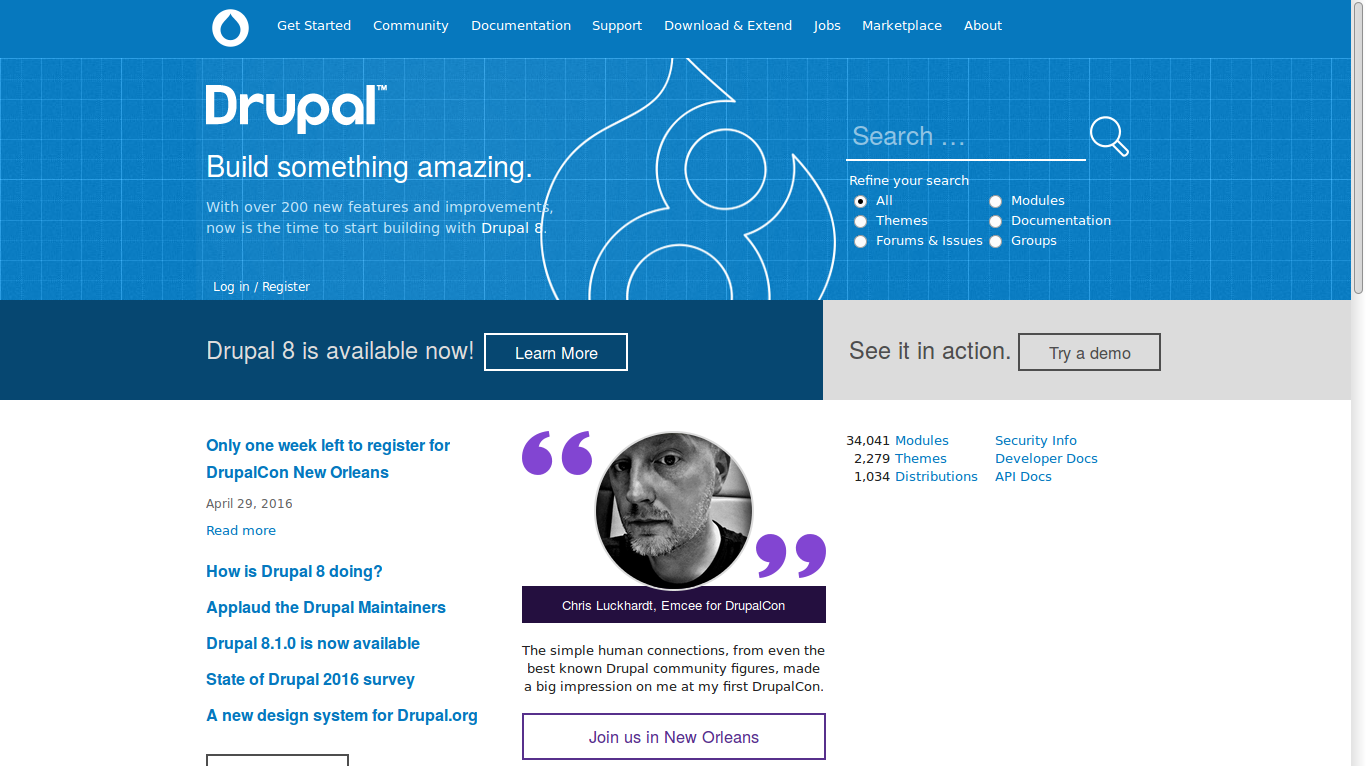
\includegraphics[width=1\textwidth]{cms-drupal-org.png}
	\caption{A drupal.org főoldala}
\end{figure}

A (\href{https://www.drupal.org/}{Drupal}) leginkább a nagyvállalatok vagy intézmények körében elterjedt. Rendkívül sokoldalú, ám hatalmas tárigénnyel rendelkezik. Tekintettel arra, hogy a telepítést követően az alap adatbázis is már önmagában több megányi adatot tartalmaz, a rendszer első használat előtti teljes körű megismerése sok időbe és energiába telik. Leginkább állami, önkormányzati vagy iskolai weboldalak kiszolgálására használják.

A \href{https://www.drupal.hu/kezikonyv/tkr}{Drupal.hu leírása}:

\begin{quote}
"A Drupal 2001. január tizenötödikén kezdte meg nyílt működését, amikor Dries Buytaert publikálta első verzióját az interneten. A rendszer azóta nagyon sokat fejlődött, és széles körben használt tartalomkezelővé vált.

\dots

A Drupal egy eléggé vékony réteget biztosít a PHP nyelvi elemei felett, mely jelentősen meg tudja könnyíteni általánosabb igényű web alkalmazások fejlesztését. Ilyen funkciók az általános űrlapkezelő rendszer, a vékony adatbázis kezelő réteg, a felhasználókezelő alrendszer."
\end{quote}

\newpage

\Section{Joomla}

\begin{figure}
	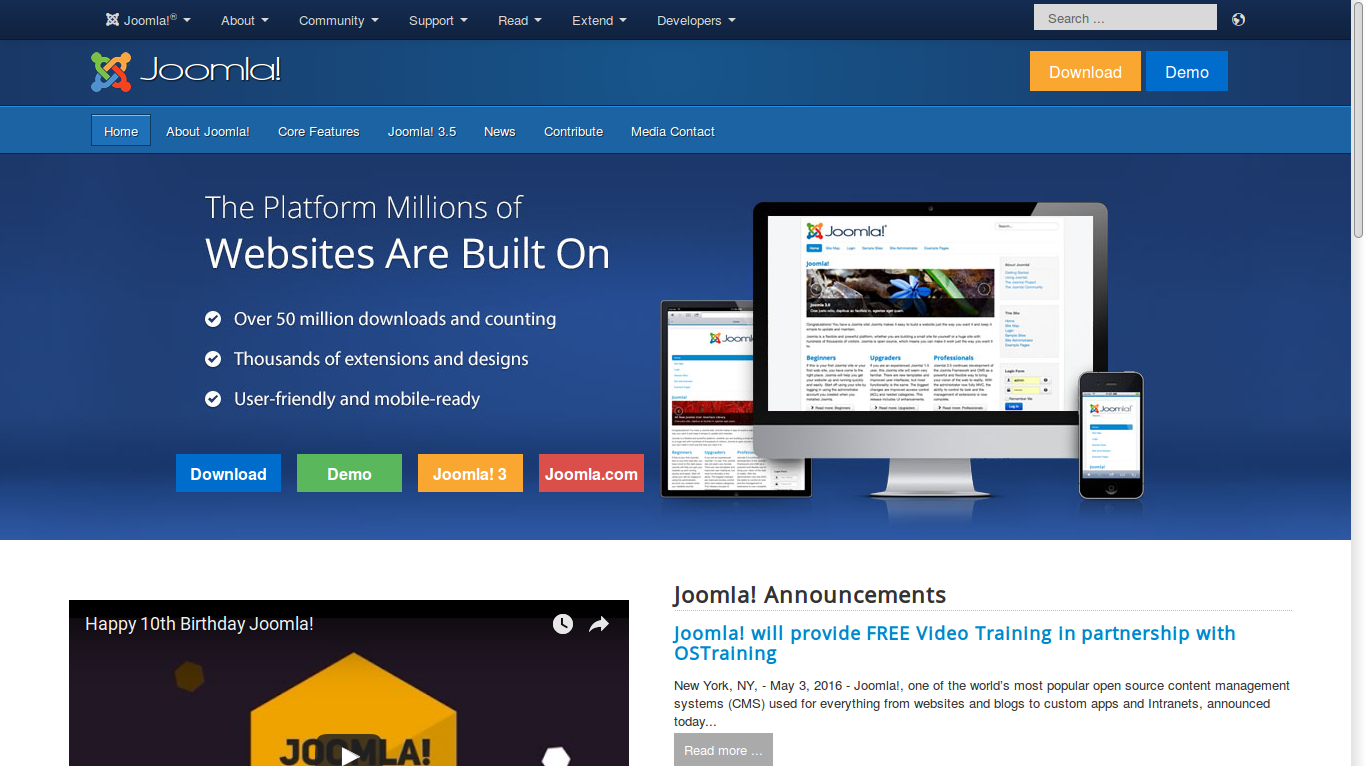
\includegraphics[width=1\textwidth]{cms-joomla-org.png}
	\caption{A joomla.org főoldala}
\end{figure}

A több, mint 50 millió letöltéssel rendelkező \href{https://www.joomla.org/}{Joomla} talán a második leginkább keresett honlapmotor. A szoftver filozófiája az, hogy az adminisztrációs felületen keresztül, külön programozás nélkül is számos feladatot el lehessen végezni. Nem véletlen tehát, hogy a webfejlesztéshez kevésbé értő személyek örömmel használják e CMS-t. Ám a sokszínű megoldás alapértelmezett mivoltának van hátránya is: programozói oldalról egy-egy fejlesztés komoly szaktudást igényel. Erősen alapszik az XML-re és a névterekre, az adminisztrációs felület biztonságára pedig különösen nagy hangsúlyt fektet.

A \href{http://joomlacms.hu/joomla/mi-a-joomla}{joomlacms.hu} leírása:

\begin{quote}
"A Joomla egy ingyenes és nyílt forráskódú tartalomkezelő rendszer (Content Management System), ami saját modell-nézet-vezérlőből (MNV) és különböző népszerű webes keretrendszerek alkalmazásából áll.

Ezeknek a technológiáknak a segítségével könnyedén oszthatunk meg különböző típusú tartalmakat a világhálón és a helyi intraneten egyaránt. Maga a Joomla! objektum-orientált programozási (OOP) szemléletet követ a fejlesztők által bevezetett szoftvertervezési minta alapján, mind ezt PHP nyelven. Az adatok tárolása MySQL-ben vagy egyéb támogatott adatbázisban történik.

Maga a rendszer egy nagy közösség által fejlesztett moduláris termék, melynek a komponenseit úgy állították össze, hogy a legszélesebb körök igényeit is kielégítse, továbbá lerövidítse az üzembe helyezést, valamint a tartalom felvitelének idejét. \dots A Joomla bővítményletöltő weboldalán több ezer bővítmény várja a felhasználókat."
\end{quote}

\newpage

\Section{Magento}

\begin{figure}
	
\includegraphics[width=1\textwidth]{cms-magento-com.png}
	\caption{A magento.com főoldala}
\end{figure}

A \href{http://magento.com/}{Magento} egy eBay Inc. fejlesztésű webáruházmotor. Bár a korábbi verziókhoz készült magyar nyelvű fordítás, azok az új kiadásokkal nem, vagy nem teljesen kompatibilisek. Alapvetően két különálló fejlesztés érhető el: egy ingyenes, kevesebb szolgáltatást tartalmazó (Community Edition), és egy díjköteles verzió (Enterprise Edition). Aki komolyabb webáruházban gondolkodik, mindenképpen célszerű kipróbálnia ezt a rendszert is, hiszen rendkívül sok funkcióval bír, és nagyszerű megoldásokat alkalmaz az adminisztráció ellátásához, valamint a megfelelő üzemeltetéshez.

A \href{http://magentoshop.hu/a-magento-keretrendszerrol/}{magentoshop.hu} leírása:

\begin{quote}
"A Magento egy nyílt-forráskódú e-commerce fejlesztési keretrendszer, amelyet jelenleg több ezer fejlesztő használ és gondoz világszerte.

\dots

A Magento egy olyan portálmotor, amely kifejezetten webáruház-funkcio- nalitás magas szintű kiszolgálására készült. Egy olyan rendkívül fejlett e-kereskedelemi keretrendszer, amely ingyenesen hozzáférhető, és amelyre\\ frontend felületet fejlesztve egy rendkívül funkciógazdag webáruházat készíthetünk.

A Magento a világ egyik vezető webáruház-motorja. Több tízezer nagy terhelhetőségű, komplex webshopot szolgál ki a világ minden táján és folyamatosan fejlődik."
\end{quote}

\newpage

\Section{OpenCart}

\begin{figure}
	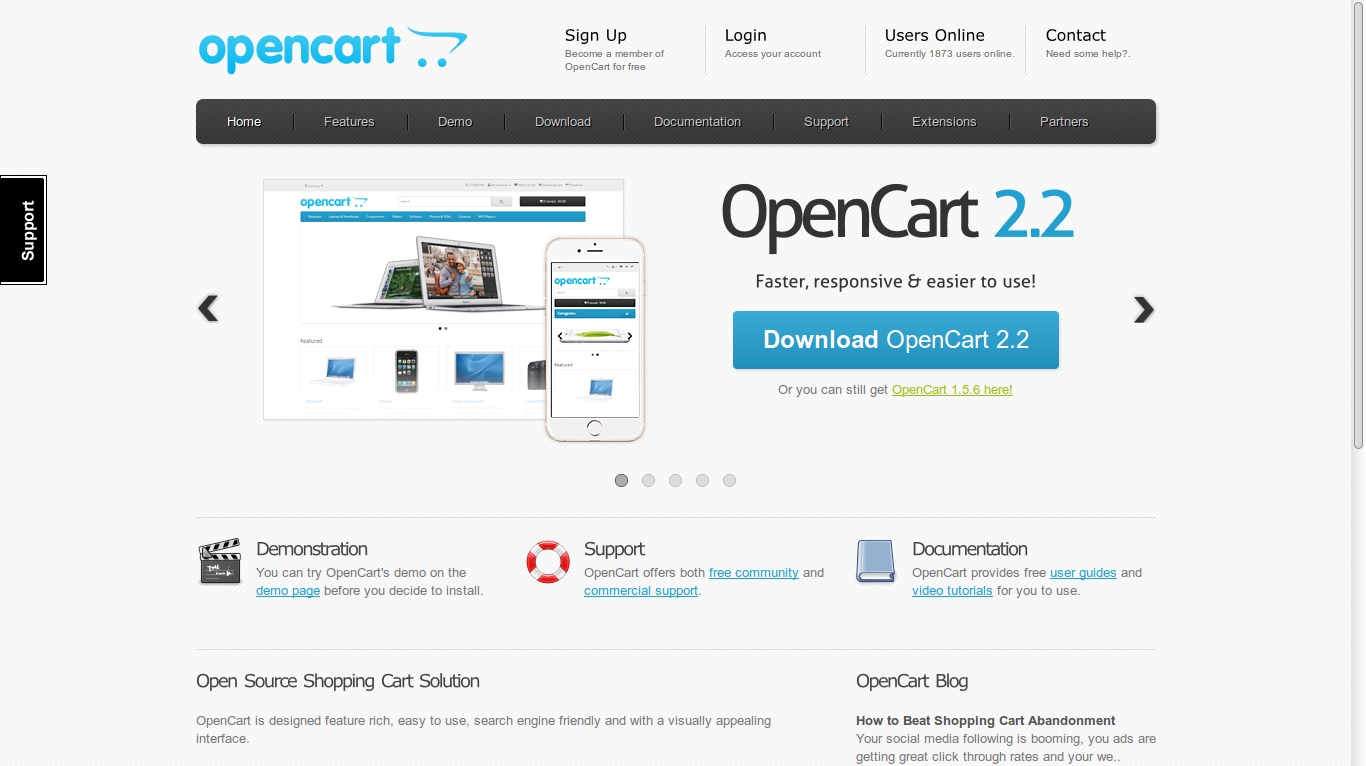
\includegraphics[width=1\textwidth]{cms-opencart-com.png}
	\caption{A opencart.com főoldala}
\end{figure}

Az \href{http://www.opencart.com/}{OpenCart} az ingyenesen elérhető webáruházmotorok közül talán a leginkább ismert és ezért leginkább használt. Bár évek óta jelen van a piacon, a második (OpenCart 2.0), már responsive verziója mégiscsak 2014. év végén jelent meg. A magyar nyelvű változat más CMS-ekkel ellentétben (Joomla, WordPress) még kevésbé kidolgozott. A szoftver talán legnagyobb hátránya, hogy tökéletesen csak webshop létrehozására alkalmas, s bár telepíthetőek különböző kiegészítők a nagyobb spektrumú használathoz, azok csak minimális szolgáltatást biztosítanak. Így például az OpenCart alapú webáruházhoz megfelelő minőségű és szolgáltatású Blog vagy Hírek aloldalt szinte lehetetlen létrehozni.

Az \href{http://www.opencart-hungary.hu/}{open-cart-hungary.hu} leírása:

\begin{quote}
"Az OpenCart egy funkciógazdag, könnyen kezelhető, keresőbarát és egy tetszetős admin felülettel ellátott webáruház rendszer.

\begin{itemize}
	\item korlátlan kategória, termékszám és gyártó kezelés
	\item többféle valuta használható
	\item többnyelvű kezelőfelület
	\item véleményezhető termékek és termék értékelő
	\item sablonokkal átváltoztatható arculat
	\item több mint 20 fizetési modul
	\item több mint 8 szállítási modul
	\item magyar nyelvű kiegészítők és modulok"
\end{itemize}
\end{quote}

\newpage

\Section{PrestaShop}

\begin{figure}
	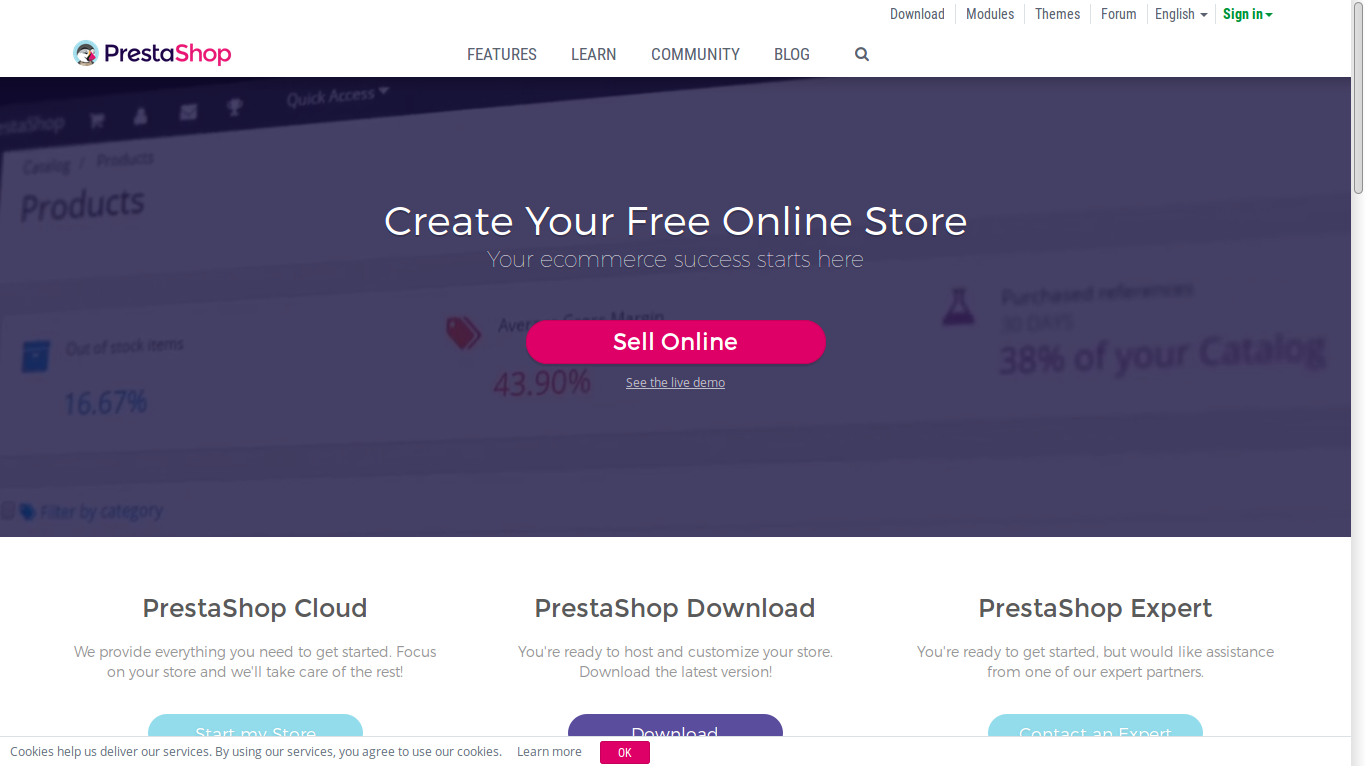
\includegraphics[width=1\textwidth]{cms-prestashop-com.png}
	\caption{A prestashop.com főoldala}
\end{figure}

A \href{http://www.prestashop.com/}{PrestaShop} webáruházmotor fejlesztését Franciaországban kezdték el, majd számos országból csatlakoztak a kezdeményezéshez, így hozva létre több nyelven is a rendszert. Egy webshop funkcióit maximálisan képes ellátni.

A \href{https://hu.wikipedia.org/wiki/PrestaShop}{Wikipédia szócikke} alapján:

\begin{quote}
	"A PrestaShop az Open Software License 3.0-s verziója alapján kiadott nyílt forráskódú e-kereskedelmi webes alkalmazás. Alapítói Igor Schlumberger és Bruno Léveque. Rugalmas és moduláris architektúrájának köszönhetően egyre nagyobb népszerűségre tesz szert. Egyszerűbb, de ugyanakkor gyorsabb, mint a Magento.

	A PrestaShop alapítása 2005-re nyúlik vissza. Öt ifjú egyetemi hallgató fogott össze az Epitech informatikai iskolában. A két nyelven (francia és angol) kiadott eredeti projektnek a phpOpenStore (POS) nevet adták. Alapítói úgy döntöttek, hogy szabad szoftverként teszik hozzáférhetővé. Számos kiskereskedő vett részt a tesztelésben és a rendszerkövetelmények meghatározásában.

	A PrestaShop felhasználói az alapkonfiguráció paraméterein kívül több szinten testre szabhatják a rendszert:
	\begin{itemize}
		\item a PHP-ismeretekkel rendelkező felhasználók az igényeiknek megfelelően tudják módosítani a programkódot;
		\item a PrestaShop felhasználói saját grafikai arculatot tervezhetnek;
		\item szolgáltatások bővítése: telepíthető, konfigurálható és szükség esetén letiltható modulok formájában lehetséges;"
	\end{itemize}
\end{quote}

\newpage

\begin{figure}
	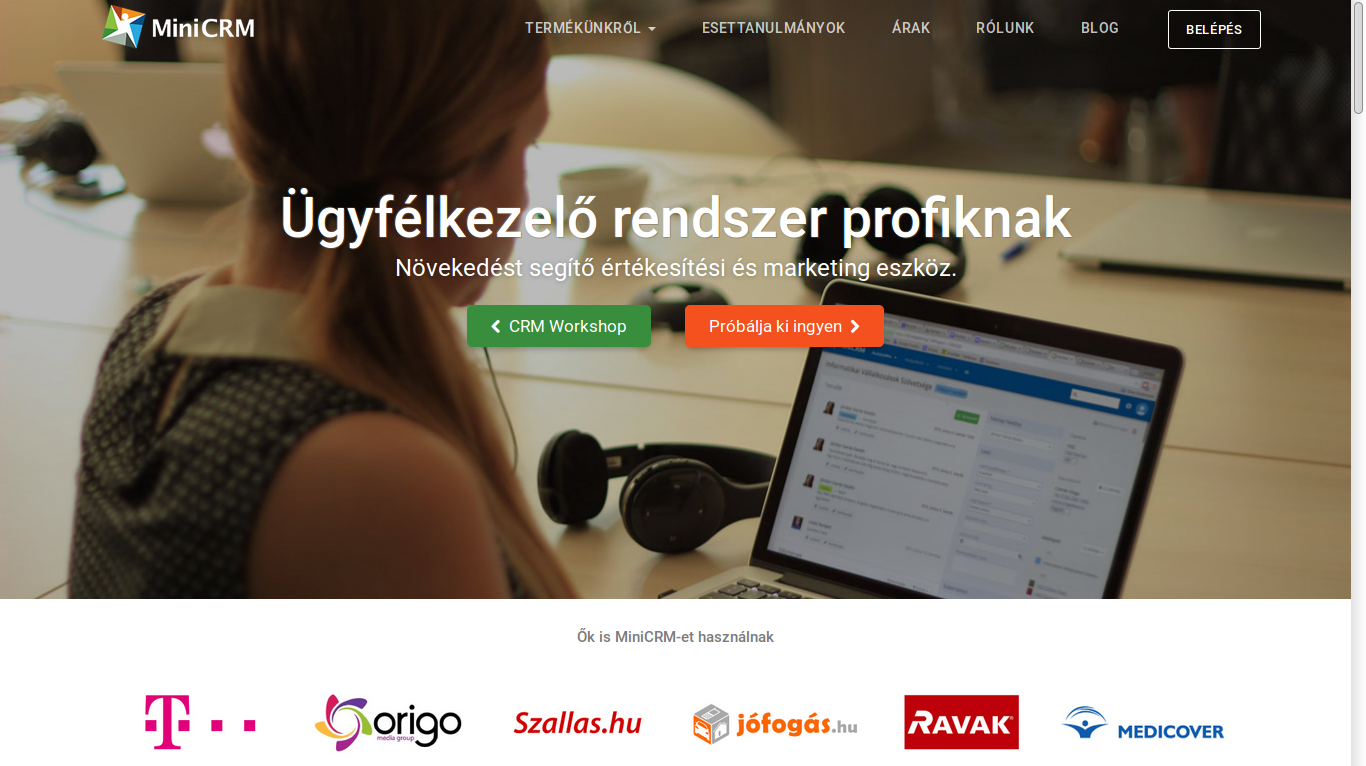
\includegraphics[width=1\textwidth]{crm-minicrm-hu.png}
	\caption{A minicrm.hu főoldala}
\end{figure}

\Section{MiniCRM}

A \href{http://www.minicrm.hu/}{MiniCRM} egy ügyfélkezelési rendszer sikeres kisvállalatoknak. Segít hatékonyan feldolgozni az érdeklődéseket, optimalizálni az értékesítési folyamatot, még több sikeres értékesítést lezárni.

Az alapítók (köztük leginkább Leskó Norbert) fejében 2006-ban fogalmazódott meg a CRM rendszer gondolata, mikor saját cégük ügyfélkapcsolatait igyekeztek a lehető leghatékonyabban kezelni. 2009 óta kizárólag a MiniCRM fejlesztésével és üzemeltetésével foglalkoznak, ami 2010-ben önálló termékként került a piacra.

A cég 2012 óta folyamatosan bővül. A munkaterületeket minden eddiginél részletesebben osztották fel, így specializálódott munkatársaik még hatékonyabban tudják segíteni ügyfeleik munkáját. A MiniCRM-et is folyamatosan fejlesztik, hogy átfogóan kielégítse a kis- és középvállalkozások igényeit.

A kitartásnak meglett az eredménye: a MiniCRM 2014-ben elnyerte a Deutsche Telekom "Legjobb üzleti app" díját, melynek köszönhetően 2015. márciustól megkezdhették terjeszkedésüket a régióban, a tervek között Horvátország, Szlovákia, Románia és Lengyelország szerepel. Ennek hála a jelenleg kizárólag magyarokból álló csapat más nemzetiségű munkatársak felvételét is tervezi.

\begin{quote}
"A CRM több, mint egy szoftver. Olyan szemléletmód, amely a vállalat legfontosabb tőkéjét állítja középpontba: az ügyfeleket. Használatával lépésről lépésre lehet a hírlevél feliratkozóból komoly érdeklődőt generálni, a komoly érdeklődőt hatékonyan lezárni, valamint a korábbi vevőknek újra eladni, egyszóval: cégértéket építeni az ügyfelekből." (forrás: \href{http://www.minicrm.hu/tour/crm/}{minicrm.hu})
\end{quote}

\newpage

\Section{Siebel}

\begin{figure}
	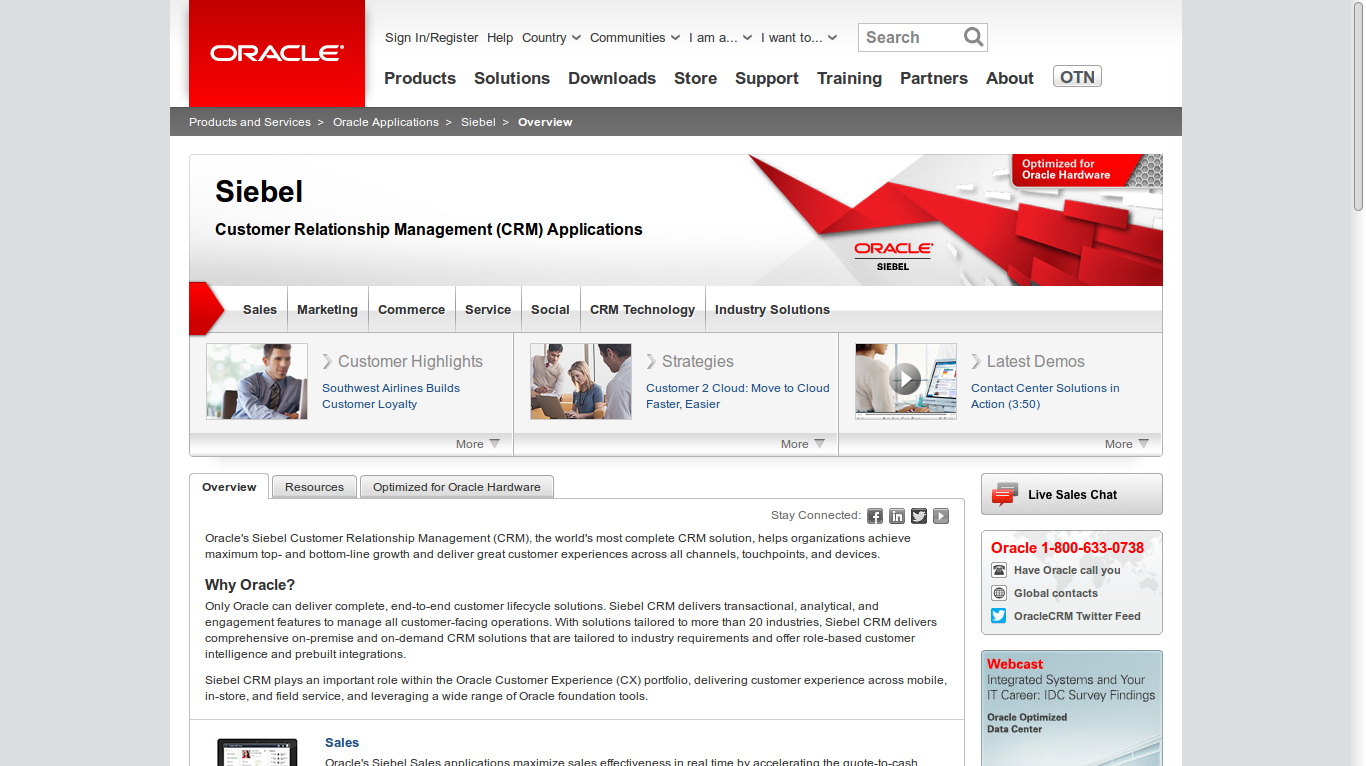
\includegraphics[width=1\textwidth]{crm-oracle-com-siebel.png}
	\caption{Az oracle.com Siebel aloldala}
\end{figure}

A \href{http://www.oracle.com/siebel}{Siebel CRM} nevét az 1993-ban alapított Siebel CRM Systems Inc. fejlesztőjéről, Thomas Siebel-ről kapta. A vállalkozást 2005-ben felvásárolta az Oracle.

A Siebel egy web-alapú megoldás az ügyféladatok nyilvántartására és kezelésére. Használata leginkább a nemzetközi nagyvállalatok körében elterjedt, mivel az alapprogram egyedi igényeknek megfelelő átalakítása jelentős költséget von maga után.

Magyarországon a Magyar Telekom Nyrt. használta hosszabb ideig, a Vodafone Magyarország Zrt. pedig évekkel ezelőtt elindította az áttérést e rendszerre.

A \href{http://www.trilobita.hu/termekek/viszonteladott-termekek/oracle-alkalmazasok/oracle-siebel-crm}{trilobita.hu} bemutatkozó leírása:

\begin{quote}
"Az Oracle Siebel CRM területen a világ egyik legátfogóbb megoldását nyújtja elsősorban olyan nagy méretű vállalatok számára, ahol a kereskedelmi és/vagy marketing tevékenység az üzleti működés szempontjából meghatározó szereppel bír.

\dots

Legfőbb referenciánk ezen a területen a Credigen Bank Zrt.-nél 2009-ben történt Siebel bevezetés, ahol a fő hangsúly a marketing kampányok teljeskörű támogatásán és az elemző funkciókon volt. A rendszert továbbá integráltuk a bank Call Center megoldásávál, ezáltal  a marketing kampányok végrehajtását is megtámogatva."
\end{quote}

\newpage

\Section{WordPress}

\begin{figure}
	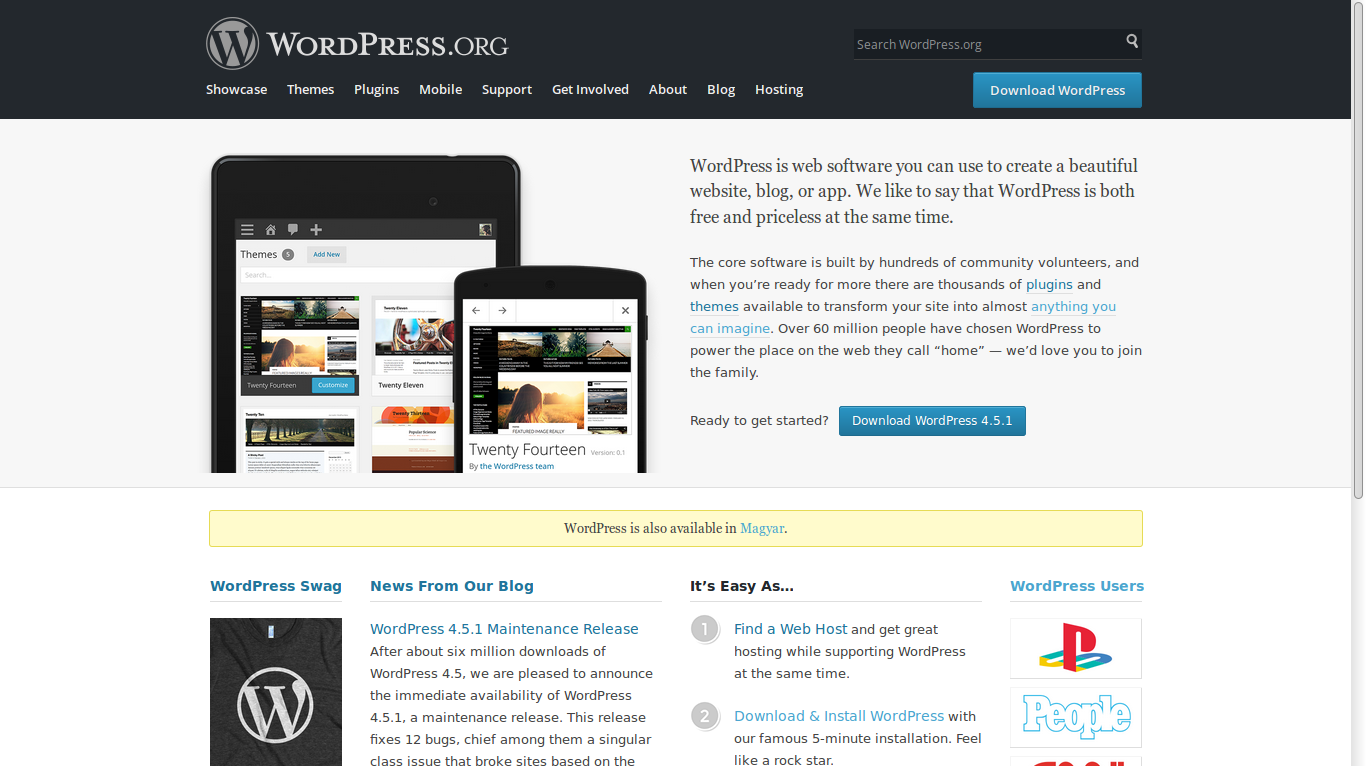
\includegraphics[width=1\textwidth]{cms-wordpress-org.png}
	\caption{A wordpress.org főoldala}
\end{figure}

A \href{https://wordpress.org/}{WordPress} napjaink egyik legelterjettebb tartalomkezelő rendszere, több tízmillió aktív weboldalt szolgál ki. Az egyedileg telepíthető eszköz a \href{https://wordpress.org/}{wordpress.org} oldalról tölthető le, míg a \href{https://wordpress.com/}{wordpress.com} honlapon egy regisztrációt követően azonnal, díjmentesen használatba is vehetjük a CMS szolgáltatásait, blogot vezethetünk, honlapot üzemeltethetünk.

A fordítások szinte minden nyelven elérhetőek, továbbá számos bővítmény (plugin) és sablon (theme/template) érhető el ingyenesen, valamint fizetős verzióban is.

A WordPress-t Matt Mullenweg (\href{http://ma.tt/}{ma.tt}), a houstoni egyetem első éves hallgatója kezdte el kifejleszteni 19 éves korában. Rendszeresen blogolt a b2/cafelog (\href{http://cafelog.com/}{cafelog.com}) alapú honlapján, ám ahogy növekedett a weboldal látogatóinak száma, egyre inkább szükségét érezte egy megbízhatóbb rendszer megalkotásának. 2003-ban létrehozta a WordPress (röviden: WP) első verzióját, mely mára a világ vezető blogmotorjává vált, 2012. márciusában 72.4 millió WP-alapú oldal létezett.

A \href{https://hu.wordpress.org/}{hu.wordpress.org} leírása:

\begin{quote}
"A WordPress egy modern publikációs platform, amely az esztétikát, a webes szabványokat, és a használhatóságot tartja szem előtt. A WordPress egyszerre ingyenes és szabadon felhasználható.

Egyszerűbben, a WordPress arra való, hogy publikálj, és nem arra, hogy harcolj vele."
\end{quote}

\newpage

\Chapter{Problémák elméleti megközelítése}
\label{Chap:problemak}

A feladat elvégzése során, mint ahogy az a projekteknél megszokott, számos kérdés vetődött fel, melyekre megoldást kellett találni. Egy-egy kérdéses elemre nyilvánvalóan több válasz is adható, így igyekeztem megtalálni a legmegfelelőbbet mind közül.

\Section{Használandó technológiák}

Első és legnagyobb kérdés a használandó technológiák kiválasztása. Döntésemnél figyelembe vettem azt, hogy manapság melyik mennyire elterjedt, emiatt hosszú távon is piacképes, valamint azt, hogy mennyire dokumentáltak, így könnyen találni már meglévő megoldásokat, valamint kiindulási pontot a hibaelhárítások során (debug). Emellett nem kerülhettem el azt a tényt sem, hogy a mobilos (ide értve a tabletet is) internethasználat rohamos léptekben terjed, ezért mind az adminisztrációs felület, mind a design tekintetében erre fel kell készülni.

\Section{Adatstruktúra szervezése}

A tárolandó, illetve használandó adatok esetében is vetődtek fel kérdések, így például a névnapi köszöntő megtervezésekor is. Egyrészt szerettem volna automatikus üzeneteket küldeni, tehát az év minden napjához el kellett tárolnom a hivatalos magyarországi névnapokat, ahol több is van egy nap, ott természetesen mindegyiket. Ekkor keresésnél a dátum jelentené az indexet. Emellett szerettem volna könnyíteni a felhasználók dolgát is azzal, hogy a keresztnév megadásakor automatikusan felajánlom az adott névhez társítható dátumokat (hiszen egy-egy névből nemcsak egy, hanem több névnap is lehet egy éven). Ebben az esetben a keresések során az index már maga a név lenne, s nem a dátum. Ez ellentmondáshoz vezetett.

Megoldási alternatíva több is adódott előttem. Egyrészt a switch-case szerkezet, másrészt a tömbök, harmadrészt az adatbázis. Figyelembe véve azt, hogy önmagában a magyar keresztnevekből több, mint 4000 van, a switch-case szerkezetet elvetettem, mert ebben az esetben már lassú lett volna a keresés, hisz ott az értékek nincsenek indexelve, a program egyszerű összehasonlítást végez. Azt is mérlegeltem, hogy nem olyan adatokról van szó, melyeket védeni kellene, ezért az adatbázisban történő tárolása értelmetlennek és feleslegesen biztonságosnak tűnt. Ezért a tömb mellett döntöttem, hiszen bár a PHP nyelvben nincs úgynevezett HashMap, mint más fejlett programozási nyelvekben (például Java), a tömb megvalósítása lényegében megfelel annak.